\chapter{Appendix}
\label{sec:appendix}

\section{Expert evaluation questions:}
\label{ExpertQuestions}
Questions were asked in German. \\
Fragen: \\
Wie viel Erfahrung haben Sie mit VR? \\
Haben Sie Motion Sickness? \\
Wie sinnvoll ist die momentane Explosionsansicht? Warum? \\
Was sind Verbesserungsmöglichkeiten? \\
Wie effektiv ist die Okklusionsvermeidung? \\
Wie effektiv kann der Kontext der Zellen betrachtet/erhalten werden? \\
Wie verständlich sind die Methoden? \\
Wie leicht fällt die Nutzung? \\

\begin{figure}[h]
	\centering
	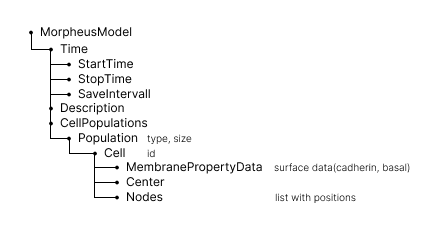
\includegraphics[width=1\linewidth]{fig/Images/DataLayout}
	\caption[]{This figure shows the structural layout of the Xml-file of the dataset. Some important attributes are written behind the name of the Xml-nodes. This figure omits many nodes that are not relevant for this work. }
	\label{fig:DataLayout}
\end{figure}

\begin{figure}[h]
	\centering
	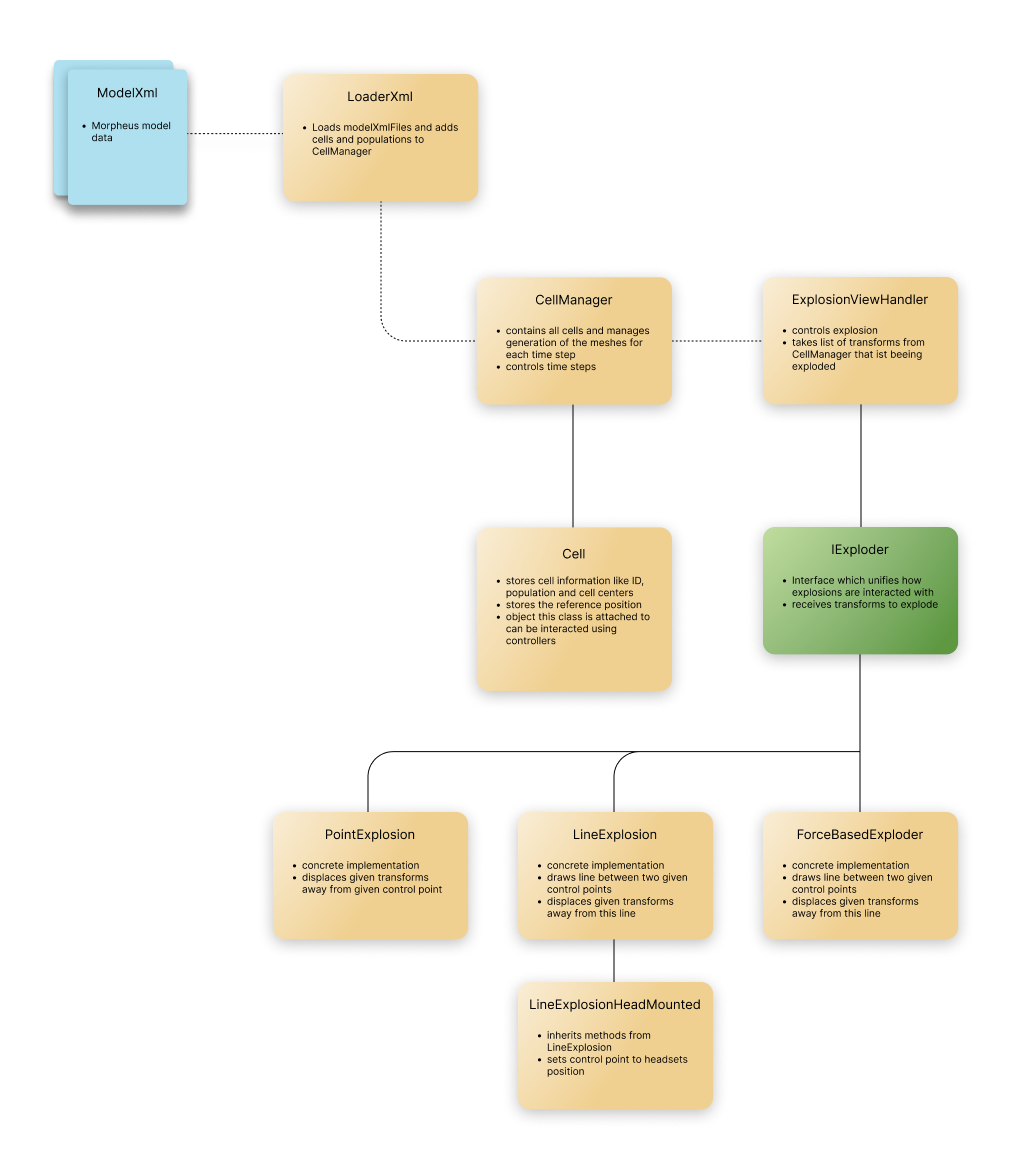
\includegraphics[width=1\linewidth]{fig/Images/objectDiagram}
	\caption[]{Object diagram of the used program structure. }
	\label{fig:objectDiagram}
\end{figure}

\begin{figure}[h]
	\centering
	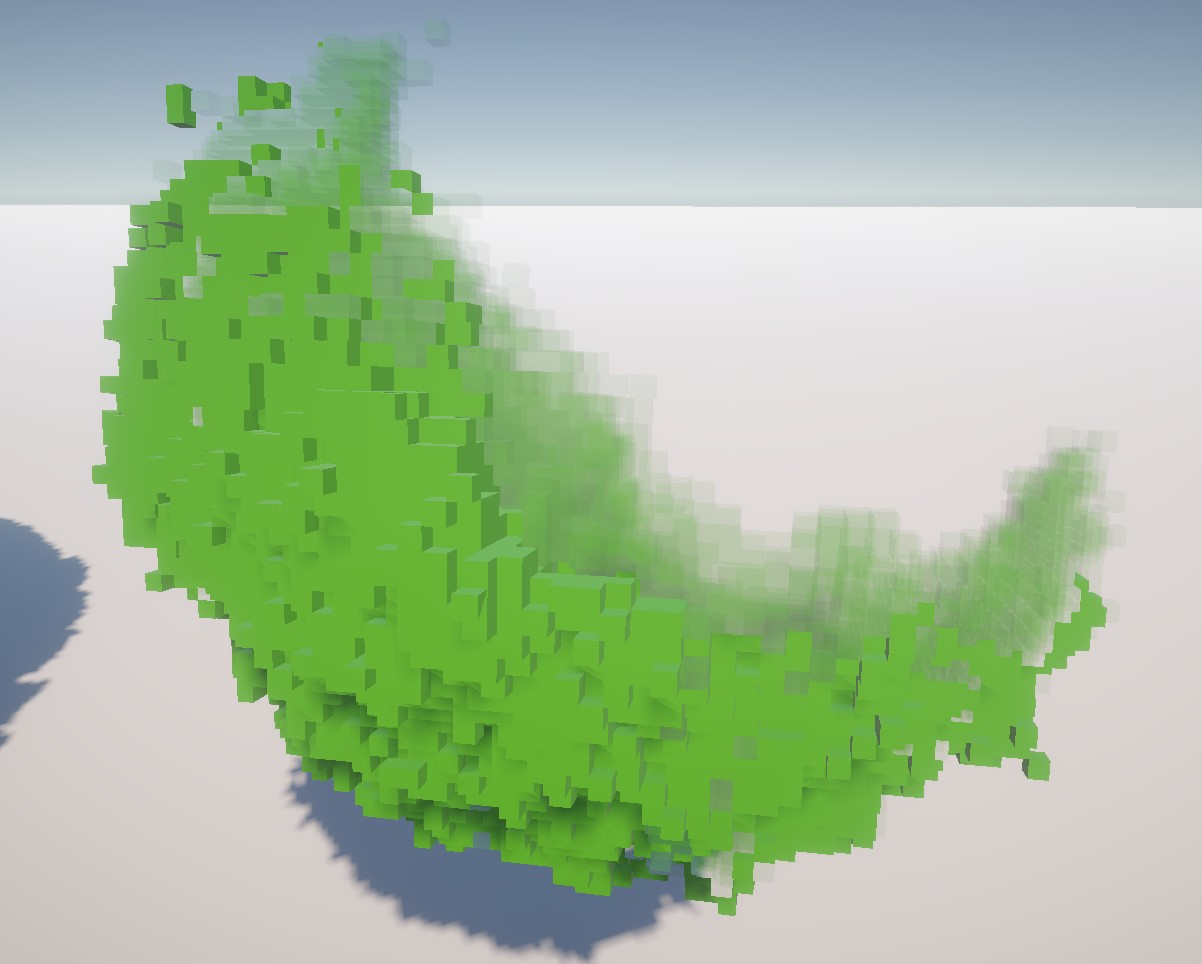
\includegraphics[width=1\linewidth]{fig/Images/ChangeOfCellTranparent}
	\caption[]{The change of a cell compared to the last time step is also shown here. }
	\label{fig:ChangeOfCellTranparent}
\end{figure}


%\chapter{Appendix II}
%\label{sec:appendix2}
%\blindtext[3]